%
% File eacl2017.tex
%
%% Based on the style files for ACL-2016
%% Based on the style files for ACL-2015, with some improvements
%%  taken from the NAACL-2016 style
%% Based on the style files for ACL-2014, which were, in turn,
%% Based on the style files for ACL-2013, which were, in turn,
%% Based on the style files for ACL-2012, which were, in turn,
%% based on the style files for ACL-2011, which were, in turn, 
%% based on the style files for ACL-2010, which were, in turn, 
%% based on the style files for ACL-IJCNLP-2009, which were, in turn,
%% based on the style files for EACL-2009 and IJCNLP-2008...

%% Based on the style files for EACL 2006 by 
%%e.agirre@ehu.es or Sergi.Balari@uab.es
%% and that of ACL 08 by Joakim Nivre and Noah Smith

\documentclass[11pt]{article}
\usepackage{eacl2017}
\usepackage{times}
\usepackage{url}
\usepackage{xspace}
\usepackage{latexsym}
\usepackage[pdftex]{graphicx}

\def \eg {e.g.,\@ }
\def \ie {i.e.,\@ }
\def \al {al.\@ }
\def \etc {etc.\@ }

%\eaclfinalcopy % Uncomment this line for the final submission
%\def\eaclpaperid{***} %  Enter the acl Paper ID here

%\setlength\titlebox{5cm}
% You can expand the titlebox if you need extra space
% to show all the authors. Please do not make the titlebox
% smaller than 5cm (the original size); we will check this
% in the camera-ready version and ask you to change it back.

\newcommand\BibTeX{B{\sc ib}\TeX}

% TJB macros
\newcommand{\dotts}{...}
\newcommand{\gap}{$*$\xspace}
\newcommand{\ex}[1]{\textit{#1}\xspace}
\newcommand{\termdef}[1]{\textbf{#1}\xspace}
\newcommand{\termemph}[1]{\textit{#1}\xspace}

\newcommand{\figref}[2][]{Figure#1~\ref{#2}\xspace}


\title{Unsupervised acquisition of comprehensive multiword lexicons \\ using competition in an $n$-gram lattice}

\author{First Author \\
  Affiliation / Address line 1 \\
  Affiliation / Address line 2 \\
  Affiliation / Address line 3 \\
  {\tt email@domain} \\\And
  Second Author \\
  Affiliation / Address line 1 \\
  Affiliation / Address line 2 \\
  Affiliation / Address line 3 \\
  {\tt email@domain} \\}

\date{}

\begin{document}
\maketitle
\begin{abstract}

\end{abstract}

\section{Introduction}

\section{Background and Related work}

In this paper we are attempting to identify \termdef{formulaic sequences}, following the terminology of Wray \shortcite{Wray02,Wray08}, wherein a formulaic sequence (FS) is defined as ``a sequence, continuous or discontinuous, of words or other elements, which is, or appears to be, prefabricated: that is, stored and retrieved whole from memory at the time of use, rather than being subject to generation or analysis by the language grammar.'' In other words, a formulaic sequence shows signs of being lexicalized. In computational linguistics, the most common term used to describe multiword lexical units is \emph{multiword expression} or ``MWE'' \cite{Sag02,Baldwin10}, but here we wish to make a principled distinction between at least somewhat non-compositional, strongly lexicalized MWEs and FS, a superset which includes MWEs but also (apparently) compositional linguistic formulas. This distinction is not a new one; it exists, for example, in the original paper of \newcite{Sag02} in the distinction between lexicalised and institutionalized phrases, and also to some extent in the MWE annotation of \newcite{Schneider14a}, who distinguish between weak (collocational) and strong (non-compositional) MWEs. It is our contention, however, that separate, precise terminology is useful for research targeted at either class: we need not strain the concept of MWE to include items which do not require special semantics, nor are we inclined to disregard the larger formulaticity of language simply because it is not the dominant focus of MWE research. Many MWE researchers would defensibly balk at including in their MWE lexicons and corpus annotations (English) formulaic sequences such as \ex{there is something going on}, \ex{it is more important than ever to \dotts}, \ex{\dotts do not know what it is like to \dotts}, \ex{there is no shortage of\dotts}, \ex{the rise and fall of\dotts}, \ex{now is not the time to\dotts}, \etc as well as tens of thousands of other such phrases which, along with less compositional MWEs like \ex{be worth \gap weight in gold}, come under the umbrella of FSs.



\begin{figure}[!t]
\center{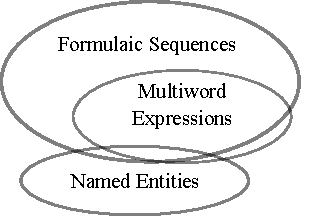
\includegraphics[width=0.35\textwidth]{FS_diagram_1.pdf}}
\caption{Multiword Terminology}
\label{fig:terminology}
\end{figure}



\figref{fig:terminology} shows our conception of the relationship between FS, MWE and (multiword) named entities. %We use the term \termdef{collocation} to refer to statistical co-occurrence without necessarily any lexicalization of the sort implied by our definition of FS. 
% TJB: I'd suggest staying away from talking about collocations altogether: it's an overloaded term; many MWEs are *not* collocations under this definition; and it's not needed for this paper
MWEs are a non-compositional subset of FS, and they overlap with named entities (NEs). In this regard, we disagree with the MWE annotation schema of \newcite{Schneider14a} which includes any NE as an MWE, which, in the context of product reviews from the Web Treebank, means that that named entities form nearly 50\% of the MWEs types attested in that corpus, with many being phrases such as \ex{Tintman Nationwide Tints Ltd} or \ex{Hickory Furniture Mart} which are easily identifiable as NEs based on their form, but would not be considered part of the mental lexicon of even a tiny fraction of English speakers.% (not even, we might argue, most of these people who work for these businesses, they likely refer to them using shorter, informal names). 
% TJB: too subtle/controversial a point for this paper
The upshot of this choice that a significant portion of ``MWE'' identification in the dataset is in fact named entity recognition. Some well-known named entities are obviously good MWEs (\eg \ex{George Washington}, \ex{the United States}), but not the names of the vast majority of people, businesses, or products which have real-word referents; they do not belong in a lexicon of formulaic sequences which is intended to reflect the internal lexicon of (at least) a significant generalizable subset of English speakers, putting them outside the scope of this work.

Regardless of the terminology used to describe them, the starting point for multiword lexicon creation has been typically lexical association measures \cite{Church90,Schone01,Evert04,Pecina10,DeAraujo11,Kulkarni11}; when these methods are used to build a lexicon, particular syntactic patterns and thresholds for the metrics are typically chosen. Only some of these measures generalize beyond two words, for example PMI \cite{Church90}, the log ratio of the joint probability to the product of the marginal probabilities. Other measures specifically designed to address sequences of larger than two words include the $c$-value \cite{Frantzi00}, a metric designed for term extraction which weights term frequency by the log length of the $n$-gram while penalizing $n$-grams that appear in frequent larger ones, and mutual expectation \cite{Dias99}, which produces a normalized statistic that reflects how much a candidate phrase resists the omission of any particular word. The lexical predictability ratio (LPR) of Brooke et \al \cite{Brooke15b} is a association measure intended for any possible syntactic pattern which is calculated by discounting syntactic predictability from the overall conditional probability for each word given the other words in the phrase. Though most association measures involve only usage statistics of the phrase and its subparts, the DRUID measure is an exception which uses distributional semantics around the phrase to identify how easily $n$-gram could be replaced by a single word \cite{Riedl15}.

Other research in MWEs has tended to be rather focused on particular syntactic patterns, looking at, for instance, just verb/noun combinations \cite{Fazly09}. The recent work of Schneider et \al \shortcite{Schneider14b} is a rare example of a comprehensive MWE identification model which distinguishes a full range of MWE sequences in the English Web Treebank, including those involving gaps, using a supervised sequence tagging model; like other models in this space, Schneider et \al make use of existing manual lexical resources and they note that an (unsupervised) automatic lexical resource could be useful addition to the model, though attempts to do so have be mixed \cite{Riedl16}. Otherwise, gaps in MWEs have generally addressed by using full syntactic representations \cite{Seretan11}.

Beyond association metrics, other general unsupervised approaches to the multiword unit identification include that of Newman et \al \shortcite{Newman12}, who used a generative Dirichlet Process model which jointly creates a linear segmentation of the corpus and a multiword vocabulary. Gimpel and Smith \shortcite{Gimpel11} focus specifically on deriving word sequences with gaps using a generative model, with the intent of improving machine translation. The drawback to these generative methods, relative to association metrics, is scalability and lack of determinacy. Brooke et \al \shortcite{Brooke14a,Brooke15b} developed a heuristic method intended for general FS identification in  larger corpora, first using the conditional probably statistics to do an initial (single pass) coarse-grained segmentation of the corpus, followed by a pass through the resulting vocabulary, breaking larger units into smaller ones based on marginal and conditional probabilities. 

%Within corpus linguistics, multiword sequences are studied with the use of \textit{lexical bundles} \cite{Biber04}, which are simply $n$-grams that occur above a certain frequency threshold. In order to get very reliable phrases, the threshold is typically set high enough (Biber et \al use 40 occurrences in 1 million words) to filter out the vast majority of expressions in the process. Lexical bundles generally involve larger phrasal chunks that would be missed by traditional collocation extraction, and so research in this area has tended to focus on how particular formulaic phrases (\eg \textit{if you look at}) are indiciative of particular genres (\eg university lectures).  Lexical bundles have been applied, in particular, to learner language: for example, Chen and Baker \shortcite{Chen10} showed that non-native student writers use severely a restricted range of lexical bundle types, and tend to overuse those types, while Granger and Bestgen \shortcite{Granger14} investigate the role of proficiency, demonstrating that intermediate learners underuse lower-frequency bigrams and overuse high-frequency bigrams relative to advanced learners. 



%Unlikely with true MWEs there is no other single necessary condition for some collection of words to be a formulaic sequence, but there are many indicators: Wray \shortcite{Wray08} lists 11 diagnostic criteria, including exact repetition, a lack of semantic transparency, genre associations, pragmatic effects, non-standard syntax, statistical irregularity, and phonological properties. We also want to distinguish FS from collocations, which are 





%Wray's conception of formulaic language is explicitly not that of mere exception to the combinatorial creativity of syntax and semantics; she argues that most language can be viewed to some degree as formulaic, and that the use of formulaic sequences is the default mode for most genres, both written and oral. Moreover, her view is that the processing of language in general should be viewed not so much as a bottom-up construction of larger phrases from individual lexical units, but rather as a top-down process where larger chunks are split apart and analyzed as discrete parts only when there is clear evidence for flexibility, a strategy that has a direct analogy in the decomposition approach used here. Another important aspect of the theory is a focus on the linear sequence rather than some other kind of syntactic abstraction (\eg a dependency relationship) as being primary to the internal representation of multiword phenomena, a perspective which allows for much cleaner analysis of longer and more varied expressions: when cases of sequence-internal flexibility occur, they are handled by the inclusion of a slot or gap which is also part of the sequence. Note that, since humans are fairly skilled at interpreting noisy input of various kinds, the notion of sequence as the default glue of the internal multiword lexicon does not rule out the possibility of greater creativity (\eg reversing word order), but this should be understood as the speaker abandoning one of the benefits of formulaic sequences (easy processing) for other communicative purposes (\eg humor).






%Second language acquisition is one of the major areas of application for work on formulaic sequences \cite{Ellis08}. Wray \shortcite{Wray08} posits that the difficulty many adult second language learners have reaching fluency reflects, at least in part, an inattention to the role of formulaic sequences, coupled with an expectation that a language should allow for free combination of words governed only by the basic rules of syntax. Modern communicative approaches to teaching tend to encourage learners to express themselves freely so long as they are able to make themselves understood, \ie to satisfy the short-term communicative goal. However, if full fluency and social integration into the culture of native speakers is a long-term goal, as it is for many immigrant learners for instance, these learners also need to correctly process and eventually produce a wide range of formulaic sequences. Creating high-coverage vocabularies based on real, modern language usage is a first step in helping learners with these challenging but ubiquitous units of language.


\section{Method}

The starting assumption for this work is that given a large corpus, a fairly low $n$-gram frequency threshold, and an extraction technique which allows for non-contiguous $n$-grams, we can collect a set of initial $n$-grams types which include a significant portion of the formulaic sequences (FS) that we can reasonably hope to identify in such a corpus; of course, the resulting vocabulary will be specific to the language, genre and domain, and there will be insufficient statistics to identify FS that are extremely rare in the corpus. Our method for FS extraction assumes such a initial set of $n$-grams, and focuses on identifying the true FS, and excluding those sequences which can be explained away due to the syntax of the language and/or the existence of other FS. The former can be captured to some extent using a syntax-sensitive association measure like LPR, but the latter requires a full, iterative model, where $n$-grams in essence complete with each other to form a compact, parsimonious formulaic vocabulary.

Our approach to FS identification involves optimization of the total cost of a lattice where each node corresponds to an $n$-gram type derived from a large corpus. The cost of the whole lattice is defined simply as a product of the costs of the individual nodes. Each node can be considered either ``on'' (is an FS) or ``off'' (is not an FS), with the base cost of being off simply a variation on the LPR association measure. Most fundamentally, $n$-gram nodes in the lattice are directionally connected to nodes consisting of $n+1$-grams which subsume them and $n-1$-grams which they subsume: that is, the (gapped) $n$-gram \ex{keep \gap under wraps} would, for instance be connected ``upwards'' to the node \ex{keep everything under wraps} and connected ``downwards'' to \ex{under wraps}. These directional relationships allow for two basic effects between nodes in the lattice when a node is turned on: \termdef{covering}, which inhibits nodes below (subsumed by) a turned-on node (\eg, if \ex{keep \gap under wraps} is on, the model will tend not to choose \ex{under wraps} as an FS); and \termdef{clearing}, which inhibits nodes above a turned-on node (\eg, if \ex{keep \gap under wraps} is on, the model would avoid selecting \ex{keep everything under wraps} as an FS). A third, undirected mechanism is \termdef{overlapping}, where nodes inhibit each other due to (non-subsuming) overlaps in the corpus (\eg having both \ex{keep \gap under wraps} and \ex{be keep \gap under} as FS will be avoided). Given these relationships, we minimize the cost of the entire lattice by iterating over the nodes and greedily optimizing the on/off choice relative to the local neighborhood of each node, until convergence.

\subsection{Collecting statistics}

The first step in the process is derive a set of $n$-grams and related statistics from a large untagged corpus of text. Since our primary association measure is an adaption of LPR, our approach in this subsection mostly follows Brooke et \al \shortcite{Brooke15b} up until the last stage. An initial requirement of any such method is a $n$-gram threshold cutoff, which for us (like Brooke et \al 2015) is 1 instance per 10 million words; we have done a manual analysis using the MWE corpus of \cite{Schneider14a} which indicates very good (over 90\%) type-level coverage excepting those highly particular proper names which would be better handled by a named entity recognition system. Note that our $n$-grams also include gappy versions; the definition of gaps is language specific, and we will discuss the individual languages further in section XXXXX. In general, though, putting in a restriction of this sort is important because it greatly lowers the number of gappy $n$-gram types. We also lower our number of types generally by excluding punctuation and by lemmatizing.  Note that as long as the count threshold is signifcantly above 1, efficient extraction of all $n$-grams can be done iteratively (one pass through the corpus per $n$) for both types in combination. 

Once a set of relevant $n$-grams is identified (and counted), other statistics required to calculate \termdef{Lexical Predictability Ratios} (LPR) for each word in the $n$-gram are collected. Again, LPR measures how statistically unlikely a particular word is relative to how predictable the word is given the same amount of syntactic context. Formally, the LPR for some word $w_i$ in the context of a sequence of words of length $n$ which have a corresponding set of sequence of POS tags $t$, is given by:

\begin{displaymath}
LPR(w_i,w_{0,n}) = \max_{0 \leq j < k < n }{\frac{p(w_i|w_{j,k})}{p(w_i|t_{j,k})}}
\end{displaymath}

These conditional probabilities can be derived in the standard way from $n$-gram and POS $n$-gram counts. We can use the same equation for gap $n$-grams, with the caveat that quantities involving sequences which include the location where the gap occurs are derived from special gapped $n$-gram statistics, not regular $n$-gram statistics.  

In Brooke et \al \shortcite{Brooke15b}, LPR for an entire span is calculated as a product of the individual LPRs, but this is not an appropriate choice here: instead, the base ``off'' cost for a node in our lattice is the minimum LPR across the words in the sequence (minLPR):

\begin{displaymath}
minLPR(w_{0,n}) = \min_{0 \leq i < n }{LPR(w_i,w_{0,n})}
\end{displaymath}

The use of minimum here should be understood in the context of competition between nodes in the lattice: minLPR for a particular $n$-gram does not reflect the \emph{overall}
degree to which an $n$-gram holds together, instead it focuses on the word which is its weakest link. For example, in the case we are evaluating the quality of \ex{be keep \gap under} as an FS, a general statistical metric might give it a high score due the strong statistical relationship between \ex{keep} and \ex{under}, but the minLPR is focused on the weaker relationship between \ex{be} and \ex{keep \gap under}.

% Some sample minLPR values are given in Table XXXXX (???). 

\subsection{Node cost functions}

For each node, there are two cost functions, one which is used if the node on ($C_{1}$), and the other if the node is off ($C_{0}$). The base value of $C_{0}$ is the minLPR metric discussed above. The base value of $C_{1}$ is a parameter to the model which, for nodes not influenced by one of the other factors discussed below, is equivalent to an initial threshold for building a vocabulary using the minLPR association measure. The lower bound on both costs is 1. There is no necessary upper bound on $C_{1}$, but we note here that there is a fairly small range of good choices for $C_{1}$; we have found that setting it too high ($>5$, corresponding to being five times more likely than predicted by POS context alone) will restrict the model primarily to sequences with only open-class words, while setting it too low ($<3$) will allow in too much random noise.

In general, we will be expanding these cost functions by adding exponential terms, reflecting the fact we do not want to override the association measure, but rather modulate it. Most of these modulations we use here are related to the node interactions discussed below, but we begin by introducing a simple example of a modulation which uses the $n$-gram count. First, lets define $C_0$ as the minLPR based taken to the power of some as yet undefined function $d_0$:

\begin{displaymath}
C_0(t) = minLPR(t)^{d_0(t)}
\end{displaymath}

LPR is a association measure based on conditional probability, and therefore tends to underestimate the importance of marginal probability, missing common expression formed using high frequency words. As such, it is common for more complex association measures to include multiplication by the count, or logarithm of the count. In the context of this model, multiplying our cost by even the logarithm of the count would be far too extreme, but we can give apply a more restricted increase to $C_0$, forcing the model to give more weight to relatively common expressions, as follows: Let $c(\dot)$ be the count function, and $c(min)$ and $c(max)$ refer to the lowest and highest count $n$-gram in the lattice (not including unigrams). 

\begin{displaymath}
d_0(t) = 1 + \frac{\log\frac{c(t)}{c(min)}}{\log\frac{c(max)}{c(min)}}
\end{displaymath}

This logarithmically scales the count into the range of 0 and 1; the $C_0$ of $n$-grams at the cutoff will be unaffected ($mod(t) = 1$) , while the maximum value of $d_0$ results in a squaring of the initial LPR-ratio.

\begin{figure*}[!tb]
\center{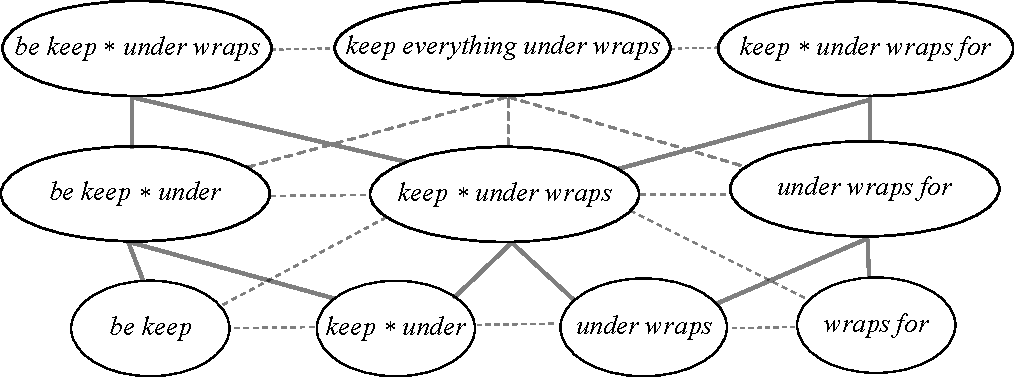
\includegraphics[width=0.8\textwidth]{FS_diagram_2.pdf}}
\caption{A portion of an $n$-gram lattice. Solid lines indicate subsumption, dotted lines overlaps}
\end{figure*}

\subsection{Node interactions}

The most important node interaction is \termdef{covering}, which corresponds to discounting or entirely excluding a node based on the presence of a node higher in the lattice. Our model includes two types of covering: hard and soft. Hard covering is based on the idea that, due to very similar counts, we can reasonably conclude that the presence of $n$-gram in our statistics is a direct result of the other: if we have 143 counts of \ex{keep \gap under wraps} and 152 counts of \ex{under wraps}, the presence of \ex{keep \gap under wraps} almost completely explains \ex{under wraps}, and it is better if we collapse these two decisions into one. We do this by permanently disabling any covered node, and giving the covering node the maximum minLPR among all the nodes it covers; this means that longer $n$-grams with function words (which often have lower minLPR) can benefit from the strong statistical relationships between open-class lexical features in $n$-grams that they cover. This is done as a preprocessing step, and besides being effective it also greatly improves the tractability of the iterative optimization of the lattice. Of course, a threshold for hard covering must be chosen: empirically, we have found that a ratio of $2/3$ (corresponding to a significant but not overwhelming majority of the counts of a lower node corresponding to the higher node) works well. Finally, we also use hard covering to partially address the rather challenging problem of pronouns, which, due to pragmatic biases in particular corpora, often have higher than desirable LPR ratios, but cannot reasonably be excluded either since many common FS contain them. In our model, $n$-grams with pronouns are considered covered (inactive) unless they cover at least one other node which does not have a pronoun.

Soft covering is used in cases when a single $n$-gram does not entirely account for another, but a turned-on $n$-gram to some extent may explain some of the statistical irregularity of one lower in the lattice. For instance, \ex{keep \gap under} is not hard-covered by \ex{keep \gap under wraps} (since there are FS such as \ex{keep \gap under surveillance}, \ex{keep it under your hat}, \etc), but if \ex{keep \gap under wraps} is tagged as an FS, we nevertheless want to discount the portion of the \ex{keep \gap under} counts that correspond to \ex{keep \gap under wraps}. We accomplish this by lowering the turned-off cost function of \ex{keep \gap under} (and thus making turning on less desirable) in the following manner: let $t$ be the target node, and $s_1\dotts_m$ be any turned-on nodes which are above $t$ in the lattice. Then, then the new $d_0$, $d_0'$ for a node $t$ is:

\begin{displaymath}
d_{0}'(t) = \frac{c(t) - \sum{c(s_1)\ldots c(s_m)}}{c(t)} d_0(t)
\end{displaymath}

\noindent
This equation is intended as a simple, quick-to-calculate approximation of the result of recalculating minLPR with the counts corresponding to the covering nodes actually removed.

In general, covering prefers turning on longer, covering $n$-grams since doing so lowers the turned-off cost function of nodes lower in the lattice. Not surprisingly, it is important to have a mechanism working in opposition, \ie one which generally prefers shorter $n$-grams. \termdef{Clearing} does this by changing the $C_0$ of nodes higher in the lattice when a lower node is turned-on. The basic mechanism is the same as covering, except that we cannot make direct make use of counts in the same way; whereas it makes sense to discount the turned-off cost of covered nodes in proportion to the (lower) relative counts of their covering nodes, in the reverse direction this logic entirely fails. A simple but effective solution is make use of the minLPR value: in this paper, we consider two options: a hard clearing where any turned-on node will clear (set $C_{0}$ to 0 for) any node higher in the lattice which has a minLPR that is lower than it; and a soft clearing which lowers  $C_{0}(t)$ based on the ratio between the minLPR for the two relevant nodes, \ie

\begin{displaymath}
C_{0}'(t) = max(1, C_{0}(t) \prod{\frac{minLPR(t)}{minLPR(s_i)})}
\end{displaymath}
where $s_i$ is the $i$th clearing node. We refer to this mechanism as clearing because it tends to clear away a variety of trivial uses of common FS which many have higher LPR due to the lexical and syntactic specificity of the FS. To give an example of its effect, if the node \ex{keep \gap under wraps} is turned on, then, assuming that their minLPR is lower, under hard clearing the $C_0$ of nodes such as \ex{be keep \gap under wraps} and \ex{keep \gap under wraps for} will be set to 1. This dissuades (but does not prevent) the model from turning on these nodes. Note that the effect of both covering and clearing is to lower the cost function for covered/clears nodes, which encourages the model to turn an $n$-gram like \ex{keep \gap under wraps} on, even supposing its minLPR were relatively low.

The third mechanism of node interaction involves $n$-grams which overlap in the corpus. Though there are some token-level exceptions (\eg coordinated compound nouns), it is generally the case that independent formulaic sequences do not overlap. For example, given that \ex{be keep \gap under} and \ex{keep \gap under wraps} often appear together, overlapping on the tokens \ex{keep \gap under}, we do not want both being selected as an FS, even in the case where both had high minLPR. To address this problem, we use a mechanism somewhat different than above: rather than lowering the off-cost, we raise the on-cost. Let $oc(x,y)$ refer to number of times nodes $x$ and $y$ overlapped in the corpus, and $o_1\dotts o_m$ refer to \termemph{turned-on} nodes which overlap with our target node $t$. With analogy to $d_0$ above, we define an $d_1$ exponential term for our target node $t$ as:

\begin{displaymath}
d_{1}(t) = \frac{c(t)}{c(t) - \sum{oc(o_1)\ldots oc(o_m)}}
\end{displaymath}

The effect of overlaps on the cost is hyperbolic: small amounts of overlapping has little effect, but with significant overlap the cost becomes prohibitive, effectively forcing one of nodes to turn off. The idea behind lowering the cost when covering and clearing is to encourage the model to turn on nodes which effectively explain the presence of nodes above and/or below it in the lattice, but we do not want to encourage nodes that just happen to overlap with others; a penalty is a more appropriate mechanism.

 
\subsection{Optimization}

The interaction between nodes discussed in the preceding section prohibit a global optimization of the lattice. Fortunately, though a majority of nodes in the lattice are connected to each other though some path, most of the effects of nodes on each other are relatively local, and effective local optimizations can be made tractable by applying some simple restrictions. The main optimization loop consists of iterations over the lattice until complete convergence (no changes in the final iteration). For each iteration over the main loop, each potentially active node is examined in order to evaluate whether its current status is optimal given the current state of the lattice. The order that we do this has an effect on the result: among the obvious options, we have found that we get the best results by ordering our nodes by frequency, which gives an implicit advantage to relatively common $n$-grams, since they will tend to be turned on first.

%The algorithm for optimization procedure is given in Figure X (???). 

Given the relationships between nodes that we have defined above, it is obviously not sufficient to consider switching only the present node; If, for instance, one or more of \ex{be keep \gap under wraps}, \ex{under wraps}, or \ex{be keep \gap under} has been turned on, the covering, blocking, or overlapping effects of these other nodes will likely prevent a competing node like \ex{keep \gap under wraps} from being correctly activated. Instead, the algorithm identifies a small set of nodes which are the most relevant to status of the node under consideration whose status should be considered simultaneously. Since turned-off nodes have no direct effect on each other, only turned-on nodes above, below, or overlapping with the current node need be considered.  Once the relevant nodes have been identified, all (including turned-off nodes) nodes whose cost function is affected by one or more of the relevant nodes are identified, and then a greedy search is carried out for the optimal configuration of the relevant nodes starting from an `all-on' state. 

In practice, we apply the following restrictions which significantly reduce the runtime of the algorithm without sacrificing the quality of the output lexicon:

\begin{itemize}
\item The complexity of the algorithm increases exponentially with the number of ``relevant'' nodes, so we limit the total number to 5. When there are more than 5 nodes turned on in the vicinity of the target node, they are selected by ranking in terms of the relative influence on each other given by the relative change in cost functions as defined in preceding section.
\item The total number of pairwise $n$-gram overlaps in a large corpus is too big too effectively store or search, and so we exclude overlaps with a count of less than 5 from our lattice.
\item Many nodes have a minLPR which is a little larger than 1. There is very little chance these nodes will be activated by the algorithm, and so to save time we simply do not consider activating nodes with a minLPR of less than 2.
\end{itemize}

\section{Evaluation}

We evaluate our approach across three different languages including evaluation sets derived from five different corpora. In English, we follow Brooke et \al \shortcite{Brooke15b} in using a 890M token filtered portion of the ICWSM social media corpus \cite{ICWSM} tagged with the Tree Tagger \cite{Schmid95}. To facilitate a comparison with Newman et \al \shortcite{Newman12}, which does not scale up to a corpus as large as the ICWSM, we also build a lexicon and test set using the 100M token BNC \cite{BNC}, using the standard CLAWS-derived POS tags for the corpus. Lemmatization included removing all inflectional marking from both words and POS tags. For English, we took the same gap definition as used in Brooke et \al \shortcite{Brooke15b}, which includes simple nouns and portions thereof.

The other two languages evaluated are Croatian and Japanese: these two languages were selected in part because of their difference from English, and in particular their reputation for being relatively free-word order; we were interested in the challenges associated with using an $n$-gram approach in such a context. For Croatian, .... Japanese

Brooke et \al \shortcite{Brooke15b} introduced a method for evaluating formulaic sequence extraction without a reference lexicon or direct annotation of the output of a model: instead, $n$-grams are sampled after applying the frequency threshold and annotated as being either an FS or not, allowing for calculation of a proper F-score for any model. We use the earlier test set built for the ICWSM corpus, and applied the same methodology (a majority annotation from 3 trained annotators) to build a new tests sets for the BNC, and for the Japanese and Croatian corpora; our new test sets consist of 500 contiguous $n$-grams and another of 500 gapped $n$-grams for each corpus. We keep the two types separate because, although rarer, gapped FS are often excluded in relevant work, and, we think, deserve special attention.  For these test sets, we report (in Table 1) inter-annotator agreement in terms of average $f$-score across annotators, which is appropriate for highly-imbalanced class situations such as this (formulaic is considered the positive class for this and other calculations), and also provides a human upper bound. In addition, we also test the ICWSM-derived lexicon against the ``MWE'' test set from Brooke et \al \shortcite{Brooke15b} whose $n$-gram annotations (both gappy and non-gappy) are derived from the MWE annotation of Schneider \shortcite{Schneider14b}.

Our primary comparison is with the heuristic LPR model from Brooke et \al \shortcite{Brooke15b} and, for the BNC, the DP-seg model from Newman et \al \shortcite{Newman12}, though the latter only handles sequential output. Both these models have been compared against a wide range of co-occurrence measures; we do not repeat all all comparisons here, but we do consider a lexicon built from ranking $n$-grams according to our primarily measure (minLPR) as well as the standard PMI. For both association measures we choose a threshold which maximizes $f$-score. All comparisons here are subject to the same $n$-gram frequency cutoff as the main model; since the content of our test sets are linked to this $n$-gram cutoff, it is not trivial to change it.

We created small development sets for each corpus and used them to do a thorough testing of a variety of parameter settings and other options, some of which we have excluded from our  discussion here. We found that we were always able to get at least near-optimal results using a $C_1$ (the on-cost) of 4, and we do not present variations on this, nor on the use of covering, which we take as fundamental to the model. Parameters that we considered in the final comparison include modulation of the off-cost using counts \emph{+cnt}, the use of hard clearing (\emph{+hcl}) or soft clearing (\emph{+scl}), and the application of penalties for overlaps \emph{+ovr}.

\section{Results}

 \begin{table*}[!bt]
 
 \begin{center}
  \caption{ F-score for formulaic sequence identification in various test sets; LLR = log-likelihood ratio C = contiguous $n$-grams, G = gapped $n$-grams. Bold is best in column.}
 \begin{tabular}{lcccccccccccccc}

       \hline
        \hline
				& \multicolumn{8}{c}{\bf{English}} & & \multicolumn{2}{c}{\bf{Croatian}} & & \multicolumn{2}{c}{\bf{Japanese}} \\
       \cline{2-9}			
       & \multicolumn{2}{c}{\bf{ICWSM}} & &  \multicolumn{2}{c}{\bf{MWE}} & &  \multicolumn{2}{c}{\bf{BNC}} & & &  && & \\
       \cline{2-3} \cline{5-6} \cline{8-9} \cline{11-12} \cline{14-15}
           \multicolumn{1}{c}{\bf{Source}}    & C & G &   & C & G &   & C & G &  & C & G & & C & G  \\
            \hline
           \hline     
           
Human agreement & & & & & & & & & & & & & &\\
 
 \hline
LLR ranking & & & & & & & & & & & & & &\\ 
LPR ranking & & & & & & & & & & & & & &\\ 
Newman al \al (2012)  & & & & & & & & & & & & & &\\ 
Brooke et \al (2015)  & & & & & & & & & & & & & &\\ 
  \hline
	Lattice\emph{+cnt+hcl+ovr} & & & & & & & & & & & & & & \\  

	Lattice \emph{+hcl+ovr} & & & & & & & & & & & & & & \\  	
		Lattice \emph{+cnt+ovr} & & & & & & & & & & & & & & \\  
			Lattice \emph{+cnt+scl+ovr} & & & & & & & & & & & & & & \\  
				Lattice \emph{+cnt+hcl} & & & & & & & & & & & & & & \\  
			
		
            \hline
           \hline                  

 \end{tabular}

 \end{center}
 \end{table*}

%One more restriction is necessary to make the use of overlaps feasible: without any restrictions, the number of connections resulting from overlaps is too large. We resolved this problem by excluding as possible active nodes. 

%a separate analysis of the that corpus showed the contents of most gapped FS in English were simple nouns or some portion thereof; this is somewhat less true for the more free word-order langauges we are also considering, but still a usuable heuristic. 

%which be described by the following (Penn Treebank) POS regular expression:

%\vspace{3mm}
%\noindent
% PP$\,$|$\,$[(PDT)(DT)JJ*[NN$\,$|$\,$NP]*(POS$\,$|$\,$PP\$)JJ*NN*]
%\vspace{1mm}

%(Our POS tags are given by the TreeTagger)

% For our main evaluation in English, our corpus is a 890 million version of the tier 1 texts in the ICWSM 2009 blog corpus \cite{ICWSM} which has been filtered to remove duplicates and near duplicates.
\bibliography{mybib}
\bibliographystyle{eacl2017}


\end{document}

%%% Local Variables:
%%% mode: latex
%%% TeX-master: t
%%% End:
